\documentclass[10pt,twocolumn,letterpaper]{article}

\usepackage{cvpr}
\usepackage{times}
\usepackage{epsfig}
\usepackage{graphicx}
\usepackage{caption}
\usepackage{subcaption}
\usepackage{amsmath}
\usepackage{amssymb}
\usepackage{color}
\newtheorem{proposition}{Proposition}
\newtheorem{lemma}{Lemma}
\newtheorem{proof}{Proof}
\newcommand{\RR}{\mathbb R}
\newcommand{\NNN}{\mathcal N}
\newcommand{\sumi}{\displaystyle{\sum_{i=1}^n}}

% Include other packages here, before hyperref.

% If you comment hyperref and then uncomment it, you should delete
% egpaper.aux before re-running latex.  (Or just hit 'q' on the first latex
% run, let it finish, and you should be clear).
\usepackage[pagebackref=true,breaklinks=true,letterpaper=true,colorlinks,bookmarks=false]{hyperref}

% \cvprfinalcopy % *** Uncomment this line for the final submission

\def\cvprPaperID{****} % *** Enter the CVPR Paper ID here
\def\httilde{\mbox{\tt\raisebox{-.5ex}{\symbol{126}}}}

% Pages are numbered in submission mode, and unnumbered in camera-ready
\ifcvprfinal\pagestyle{empty}\fi
\begin{document}

%%%%%%%%% TITLE
\title{Square Loss Exemplar Machine as Image Encoding: Applications on Image Retrieval}

\author{Rafael Rezende\\
Institution1\\
Institution1 address\\
{\tt\small firstauthor@i1.org}
% For a paper whose authors are all at the same institution,
% omit the following lines up until the closing ``}''.
% Additional authors and addresses can be added with ``\and'',
% just like the second author.
% To save space, use either the email address or home page, not both
\and
Second Author\\
Institution2\\
First line of institution2 address\\
{\tt\small secondauthor@i2.org}
}

\maketitle
%\thispagestyle{empty}

%%%%%%%%% ABSTRACT
\begin{abstract}
   In this paper, we propose an improvement of the image encoder based on the exemplar SVM, first proposed bt Zepeda et al.
   First, we show a more efficient implementation, replacing the hinge loss by the square loss. 
   We obtain superior results on image search in a fraction of the execution time.
   Then, we introduce a low-rank kernel trick for exemplar SVM \emph{\color{red} talk about results} 
\end{abstract}

\section{Introduction}



An effective image 
representation is a crucial component of image retrieval systems
where, given some query image,  images must be retrieved from a large 
database, then ranked according to their degree of similarity with the 
query.
%Robust image representations are a crucial component of a vast number of computer vision applications. 
%Within these, the \emph{image retrieval} application is an important example wherein a query image is provided to the system, which must in turn find all matching images from within a large, unannotated database. 
The matching process is done entirely based on the pixel content of the query and database images, and the search must be robust to large image variations due to camera pose, color differences and scene illumination, amongst others.


The advances in image representation enabled the success of new systems in this challenging task. %An image representation function commonly maps a given input image to a vector in a fixed dimensional space called the image \emph{feature vector}. 
Indeed, many successful feature representations for image retrieval rely on unsupervised models such as $K$-means \cite{Delhumeau2013} or Gaussian mixture models \cite{Perronnin2010} and, before the neural networks \textit{renaissance}, these representations would outperform methods that exploit supervised learning of image features directly~\cite{Bilen2015,Rana}.
Today, with the popularization of convolutional architectures, global image descriptors are often obtained by aggregation and/or pooling the last convolutional layers \cite{babenko15,GoAlReLa16,KaMeOs16} or by addition of new differentiable layers to an existing architecture~\cite{Arandjelovic15}.
%One of the main reasons for this is the lack of adequately large and varied supervised datasets that are expensive to collect.
%A now pervasive example of an image feature representation is that consisting of the activation coefficients extracted from the previous-to-last layer of Convolutional Neural Networks (CNNs) \cite{Krizhevsky2012}. Although CNNs are trained in a fully-supervised manner for the image classification task, they have been shown to transfer well not only to new, unseen classes \cite{Oquaba,Chatfield2014}, but also to alternate tasks such as object detection \cite{Girshick2014} and, importantly, image retrieval \cite{Sharif}.

The exemplar support vector machine (ESVM), originally proposed by Malisiewicz {\it et al.} \cite{Malisiewicza}, leverages the availability of large, unannotated pools of images within the context of supervised learning. It uses a large generic pool of images as a set of negative examples, while using a single image (the \emph{exemplar}) as a positive example. Given these training sets, an SVM classifier is learned that can  generalize well, despite the drastically limited size of the set of positive examples.

Zepeda \emph{et al.} \cite{ZePe15} propose to treat instead the weights of the resulting classifier as a new feature vector for image retrieval. %This new ESVM feature is derived from \emph{base} feature representations ({\it e.g.,} CNN activation features) of the exemplar and the negative pool.
%An extension \cite{ZePe15} of the ESVM formulation discussed above instead treats the resulting  classifier as an \emph{enhanced} representation of the image feature representing the exemplar image (the \emph{base} feature representation).
An ESVM feature is extracted from each database image, as well as from the query image, by treating each image as an exemplar while keeping a fixed pool of generic negative images. Searching amounts to computing distances between the query and the database ESVM features. Note that ESVM features can be derived from arbitrary \emph{base} features ({\it e.g.}, CNN activations) of the exemplar and the images in the generic negative pool. %An interesting interpretation of this approach is that the ESVM features represent what is unique about the exemplar relative to the pool of generic negatives, which is the role of a classifier.


One important drawback of the ESVM feature encoding approach is that computing the  classifier requires solving an optimization problem for each positive example (\ie each query and each database image). This can be time consuming for the large negative pool sizes required for good ESVM feature performance. In this work we propose using the square loss instead of the hinge loss, in effect converting the ESVM problem into a ridge regression that can be solved in closed form. The parameters of the corresponding classifier, which we call the square loss exemplar machine (SLEM), had been shown to both generalize LDA \cite{Koba15} and, for the general case of multiple positive samples (LS-SVM)~\cite{lssvm}, form features with comparable binary classification performance while drastically reducing the computational cost.


Since computing the SLEM features requires inverting a large matrix related to the training set's covariance matrix, we propose an efficient way to compute this inverse that exploits the fact that only a single (positive) example changes in the training set when computing SLEM features for different images. We show experimentally that our representation matches and even improves upon the performance of ESVM features on two standard datasets using a wide range of base features.

We also introduce a kernelized variant of SLEM that enjoys similar computational advantages but improves retrieval performances. Further computational efficiency is obtained using a kernel principal components analysis (KPCA) decomposition of the negative samples.
%low rank incomplete Cholesky decomposition of the negative pool kernel matrix.

The rest of this paper is organized as follows:
%In Section \ref{prior work} we provide an overview of various existing feature representation methods. 
In Section \ref{lsesvm} we first review the original ESVM feature representation method and subsequently introduce the proposed linear SLEM model. We then introduce the kernelized SLEM variant in Section \ref{nonlinear SLEM}. We then present the low-rank approximation of our method that enables efficient implementations in the non-linear case in Section \ref{eff_imp}. We evaluate our proposed method in image retrieval in Section \ref{eval}, and present conclusions in Section \ref{conclusion}.



% Image search
% - Importance.
% - Feature representations. 

% Feature representation - supervised learning
% - Generic framework.
% - Deep CNN features.
% - ImageNet.

% Image retrieval
% - Supervised - Eusipco, NetVLAD.
% - VLAD, Fisher.
% - Cheaper.

% Pool:
% LDA
% SVMs for feature representations - parts learning, Malizsiewics


%\section {Introduction}
% The exemplar SVM (E-SVM) was first introduced by Malisiewicz et al. in \cite{Efros11} as a conceptually simple framework for object detection and image classification where the training set has a small ratio of positive/negative examples. 
% At training time, many SVMs are learned from a large pool of negative against a single positive (so called exemplar). 
% At test time, the scores of the test images for each classifier are fitted by a logistic regression. 
% The final score of an image is then a non-linear combination of scores from multiples exemplar SVMs.

% They have also been used in \cite{Efros12} in image retrieval tasks, using the classifier score to rank matching candidates.
% However this transfer of information from classification to retrieval is severely limited. 
% Indeed, the purpose of a support vector machine is to separate positive and negative samples, i.e., predict discrete labels. 
% The distance between a negative sample and the classification hyperplane has no value as a measure of has \emph{a priori} no value of continuous matching score.

% Zepeda et al. address this problem in \cite{ZePe15} by firstly, performing an E-SVM to each image in a dataset instead of only for the query images and secondly, comparing its classifiers distance to the query's classifier instead of comparing scores. 
% These modifications guarantee we are ranking distances between two points instead of classification scores.
% Therefore \cite{ZePe15} refers to E-SVMs as features encoders: a pipeline that takes an image representation as input and returns an improved image representation. This type of feature enhancing is more akin to methods such as whitening, PCA and LDA.

% This paper introduces the square-loss Exemplar machine (SLEM), which consists of optimizing the same cost function of a regular E-SVM where the hinge loss is replaced by the square loss. 
% The square loss version has the advantage of having a much more efficient optimization. Indeed, the minimization of its cost function is solved by a linear system and can be done for all exemplar simultaneously, whereas the regular E-SVM cost function is generally minimized one exemplar at a time, normally by stochastic gradient descent \cite{bottou10}.
% Also, for the machine learning tasks of binary classification, both regular SVM and least-squares SVM have similar performances \cite{YeXi07}.
% %Also, for the machine learning tasks of binary classification, both regular SVM and least-squares SVM have the same performance if positive and negative samples are separable and the pool of samples is linearly independent \cite{YeXi07}. 
% We also introduce a kernelized version of SLEM, efficiently implemented, that gives better results and superior scalability for large-scale image retrieval problems.

%%% Local Variables:
%%% TeX-master: "main_eccv"
%%% End:


\section{Prior work}

\section{Square loss exemplar machine}\label{lsesvm}
In this section, we revisit the exemplar SVM model presented by \cite{Efros11} as an instance of a more general family of classifiers. Then, we introduce the square loss exemplar machine (SLEM) by solving a simple variant this model and study its properties.
\subsection{Exemplar classifiers} \label{esvm}
We are given base features in $\RR^d$ at training time, one positive example $x_0$ in $\RR^d$ and a set of negative examples $X = [x_1, x_2,...,x_n]$ in $\RR^{d\times n}$, each column of $X$ representing one example by a vector in $\RR^d$. 
We are also given a loss function $l:\{-1, 1\}\times \RR\rightarrow\RR^+$. Learning an exemplar classifier from these examples amounts to minimizing the function 
\begin{equation}
J(\omega, \nu) = \theta \ l(1, \omega^Tx_0+\nu) +\dfrac{1}{n}\sumi l(-1, \omega^T x_i+\nu)+\dfrac{\lambda}{2}\|\omega\|^2, 
\label{eq:first}
\end{equation}
w.r.t. $\omega$ in $\RR^d$ and $\nu$ in $\RR$. In Eq. (\ref{eq:first}), $\lambda$ and $\theta$ are respectively a regularization parameter on $\omega$ and a positive scalar adjusting the weight of the positive exemplar.
%\footnote{We could also acknowledge a parameter $\theta$ other than $\frac{1}{n}$ as a regularization to the error of each negative example. But this parameters seems to be less important to cross-validate. Also, setting $\theta=\frac{1}{n}$ simplify Equation (\ref{omega:solution}) and allows the use of Woodbury identity.} 

Given a cost $l$, we define the correspondent \emph{exemplar classifiers} of $x_0$ with respect to $X$ are the weights $\omega^\star(x_0,X)$ that minimizes the loss function $J$:
\begin{equation}
\big(\omega^\star, \nu^\star\big) = \underset{(\omega,\nu)\in\RR^d\times\RR}{\argmin} \ J(\omega, \nu). \footnote{Depending on the loss function $l$, $\nu^\star(x_0,X)$ may be not unique.}
%\big(\omega^\star(x_0, X), \nu^\star(x_0, X)\big) = \underset{(\omega,\nu)\in\RR^d\times\RR}{\argmin} \ J(\omega, \nu). 
\label{omega:first}
\end{equation}
%To shorten the notation, we refer to these solutions as $\omega^\star$ and $\nu^\star$ when their arguments are implicit.

%\cite{Efros11} introduced ensembles of exemplar classifiers for object detection, but single exemplar classifiers have been used as replacement of the original feature $x_0$ for image classification and retrieval \cite{ZePe15} and detection \cite{GMPD12}. \RAF{Maybe this should be in the introduction instead.}
The exemplar SVM~\cite{Efros11,Efros12} is an instance of this model where $l$ is the hinge-loss. 
%Applications of ESVM use the hinge loss function, which guarantees that $J$ is a convex function. 
The solution of Eq. (\ref{omega:first}) can be thus found by stochastic gradient descent~\cite{bottou10} individually for each positive sample. The next subsection show how to calculate all exemplar classifiers simultaneously by changing the loss function.

\subsection{Square loss function}\label{slem:intro}
Now, let us study the same learning problem for the square-loss function $l(y,\hat{y}) = \frac{1}{2}(y-\hat{y})^2$. As in the case of the hinge loss, Equation (\ref{eq:first}) is a convex problem. 
However it is now a ridge regression problem, whose unique solution can be found in closed form as
\begin{align}
\begin{cases}
\vspace{3 mm}
\omega^\star &= \dfrac{2\theta}{\theta+1}U^{-1}(x_0-\mu), \\
%\vspace{3 mm}
\nu^\star &= \dfrac{\theta-1}{\theta+1}-\dfrac{1}{\theta+1}(\theta x_0+\mu)^T\omega^\star,
\end{cases}
\label{omega:solution}
\end{align}
%\begin{align}
%\nu^\star &= \dfrac{\theta-1}{\theta+1}-\dfrac{1}{\theta+1}(\theta x_0+\mu)^T\omega^\star, \label{eq:nustar}\\
%\omega^\star &= \dfrac{2\theta}{\theta+1}U^{-1}(x_0-\mu) \label{eq:wstar}
%\end{align}
where:
\begin{align}
\begin{cases}
\mu = &\frac{1}{n}\sum_{i=1}^n x_i,\\ \\
U = &\frac{1}{n}XX^T-\mu\mu^T\\
&+\frac{\theta}{\theta+1}(x_0-\mu)(x_0-\mu)^T+\lambda\mathrm{Id}_d. \label{eq:U}
\end{cases}
\end{align}
Equation (\ref{omega:solution}) shows how to solve (\ref{eq:first}) simultaneously for all exemplars.
\cite{lssvm}
%Replacing the hinge loss by the square loss offers a more compact solution, but not necessarily more efficient.

\textbf{Woodbury identity.} 
We can simplify Eq. (\ref{omega:solution}) by modifying $U$ in Eq. (\ref{eq:U}).
Let us define $A = \frac{1}{n}XX^T-\mu\mu^T +\lambda\mathrm{Id}_d$ our regularized covariance matrix and assume its inverse $A^{-1}$ known. 
%$A$ is the covariance matrix of the negative samples $X$\footnote{added of a small term proportional to the identity matrix to insure $A$ is positive-definite.}. Let us assume its inverse $A^{-1}$ is known. 
The matrix $U$ now reads $U = A + \frac{\theta}{\theta+1}\delta\delta^T$, where $\delta=x_0-\mu$ is the centralized (w.r.t. the negatives' mean) positive sample. The Woodbury identity \cite{woodbury} gives us
\begin{equation}
U^{-1} = A^{-1} -\dfrac{\theta}{\theta\delta^TA^{-1}\delta+ \theta+1}A^{-1}\delta^T\delta A^{-1}. \label{invU}
\end{equation}
Substituting (\ref{invU}) in (\ref{omega:solution}) yields
\begin{equation}
\begin{split}
\omega^\star &= \dfrac{2\theta}{\theta +1}\left(A^{-1}\delta - \dfrac{\theta}{\theta\delta^TA^{-1}\delta+ \theta+1} A^{-1}\delta (\delta^TA^{-1}\delta)\right)\\
&= \dfrac{2\theta}{\theta\delta^TA^{-1}\delta+ \theta+1} A^{-1}\delta.\label{Wood:omega}
\end{split}
\end{equation}

Note that the positive sample weight $\theta$ does not influence the direction of the optimal vector $\omega^\star$, only its norm. This means that if search and ranking are based on the normalized feature $\frac{1}{\|\omega^\star\|}\omega^\star$, $\theta$ does not influence the matching score of the SLEM vectors of two different images. This sets SLEM appart from ESVM which requires this parameter to be calibrated \cite{Efros11,ZePe15}. We can thus set $\theta=\frac{1}{n}$ for the remaining of this work.
%The normalized exemplar classifier $\omega^\star$ is therefore a linear transformation of $x_0-\mu$.
%Indeed, if $\omega$ and $\omega'$ are the $d$-dimensional SLEM vectors of $x$ and $x'$, respectively, their cosine similarity reads:
%we can denote $s$ the matching score scalar function defined in $\RR^d\times \RR^d$, which is given by
%\begin{equation}
%s(\omega, \omega') = \dfrac{\omega^T \omega'}{\|\omega\| \|\omega'\|} = \frac{(x-\mu)^TA^{-2}(x'-\mu)}{\|A^{-1}(x-\mu)\|\|A^{-1}(x'-\mu)\|},\label{match:score}
%\end{equation}
%which does not depend on the value of $\theta$. 
%This means that the weight of the positive sample can be fixed at any positive value without changing matching scores. 

\subsection{LDA and SLEM}\label{sec:lda}

It is interesting to note the relationship between SLEM and the classical linear discriminant analisys (LDA).
Let us reanalyse Eq. (\ref{eq:first})) an suppose that we have multiple positive samples. It can be shown that in this case, the corresponding linear classifier of Eq. (\ref{eq:first}) for the square-loss is also given by
(\ref{omega:solution}), where $x_0$ denotes this time the center of mass
of the positive samples {\em if} these samples have the {\em same} covariance matrix $\Sigma$ as the negative samples $X$.
 
This equal-covariance assumption is of course quite restrictive, and probably unrealistic in general. It is interesting to note, however, that this is exactly the assumption made by linear discriminant analysis. As shown in~\cite{Hastie2009} for example, LDA can be seen as a (non-regularized) linear classifier with decision function $\omega^T_{LDA} z+ \nu_{LDA}$, where $z$ is a sample in
$\RR^d$, and
\begin{equation}
\left\{\begin{array}{l}
\displaystyle \omega_{LDA}=\Sigma^{-1}(x_0-\mu),\\
\displaystyle \nu_{LDA}=-\frac{1}{2}(x_0+\mu)^T \omega_{LDA},
\end{array}\right.
\label{eq:lda}
\end{equation}
 
This shows that SLEM is a generalized version of LDA: Indeed, when $\lambda=0$ in SLEM (i.e. no regularization), $A = \Sigma$, the vectors $\omega_{LDA}$ of Eq. (\ref{eq:lda}) and $\omega^\star$ of Eq. (\ref{Wood:omega}) have the same direction.
%This observation has been equally made by \cite{Koba15}.
Many interesting properties of LDA has been used recently for classification tasks \cite{GMPD12,HMR12} and, more recently, for image retrieval with convolutional neural network activations \cite{babenko15}.
With our simple generalization of LDA, we hope to obtain superior results.

%In the next section, we take one step further and generalize SLEM with kernel methods. \hlc{something to add to this sentence?}


%%% Local Variables:
%%% TeX-master: "main_eccv"
%%% End:


\section{The kernel SLEM}
\label{nonlinear SLEM}

\subsection{Kernel methods}\label{kernel:review}
Let us recall a few basic facts about kernel methods for supervised
classification. We consider a reproducing kernel Hilbert space (RKHS)
$H$ formed by real functions over some set
$X$, and denote by $k$ and $\varphi$ the corresponding reproducing kernel and feature map (which may not admit a known explicit form) over $X$, respectively. We
address the following learning problem over $H\times\RR$:
%\begin{equation}
%\min_{h\in H,\nu\in\RR}
%\sum_{i=1}^n l(y_i,h(x_i)+\nu) + \frac{\lambda}{2}\|h\|_H^2,
%\label{eq:kernel}
%\end{equation}  
%By definition of a reproducing kernel,
%Equation (\ref{eq:kernel}) can be rewritten as
\begin{equation}
\min_{h\in H,\nu\in\RR}
\dfrac{1}{n}\sum_{i=1}^n l(y_i,\langle \varphi(x_i),h\rangle+\nu) +
\dfrac{\lambda}{2}\|h\|_H^2,
\label{ker:aff}
\end{equation} 
where the pairs $(x_i,y_i)$ in $X\times \{-1,1\}$, $i=1\dots n$ are training samples, %and $l: \{-1,1\}\times \RR\rightarrow\RR^+$ is some arbitrary loss function. 
%$\varphi$ is the {\em feature map} over $X$ associated with the kernel $k$ (which may not admit a known explicit form) 
and $\langle h, h' \rangle$ is the inner product of element $h$ and $h'$ in $H$. We dub problems with the general form of (\ref{ker:aff}) {\em affine}
supervised learning problems since, given some fixed element $h$ of
$H$ and some scalar $\nu$, $\langle h,h'\rangle+\nu$ is an affine function of $h'$,
whose zero set defines an affine hyperplane of $H$ considered itself
as an affine space.

Let $K$ denote the kernel matrix with entries $k_{ij}=\langle\varphi(x_i),
\varphi(x_j)\rangle$ and rows $k_i^T=[k_{i1}, k_{i2},...,k_{in}]$, $i$ in $\{1,\ldots,n\}$.  We assume from now on that $l$ is convex and continuous. Under this assumption, Eq. (\ref{ker:aff}) admits an equivalent formulation
\begin{align}
\min_{\alpha\in\RR^{n}, \ \nu\in\RR} \left(\dfrac{1}{n}\sumi l(y_i, k_i^T\alpha+\nu)  +\dfrac{\lambda}{2}\alpha^TK\alpha\right), \label{ker:first}
\end{align}
and any solution $(\alpha^\star,\nu^\star)$ to (\ref{ker:first})
provides
a solution $(h^\star,\nu^\star)$ to (\ref{ker:aff}) with
$h^\star=\sum_{i=1}^n \alpha_i^\star\varphi(x_i)+\nu^\star$. This result follows from the Riesz representation theorem~\cite{SHS01,Wahba90}.


%where $K$ is a $(n+1)\times (n+1)$  matrix and $k_i$ is its $(i+1)$-th column matrix for $i$ in $\{0, 1, ..., n\}$.\\



Assuming our reproducing kernel is semidefinite positive, 
%\footnote{\textit{i.e.} for any $z$ in $\RR^n$, $z^TKz\ge 0$. This is equivalent to all eigenvalues of $K$ being non-negative.} 
$K$ is a semidefinite positive matrix and can be decomposed as $K=BB^T$.
%, with $B$ a rank $r$ upper triangular matrix of size $n\times r$. 
Using this factorization, the kernelized problem can be expressed as 
\begin{equation}
\min_{\beta\in\RR^r,\nu\in\RR} \left( \dfrac{1}{n}\sumi l(y_i, b_i^T\beta+\nu)+\dfrac{\lambda}{2}\|\beta\|^2\right), \label{beta:first}
\end{equation}
where $b_i^T$ denotes the $i$-th row of $B$ and $r$ is the number of columns of $B$. 
If $(\beta^\star, \nu^\star)$ is the solution Equation (\ref{beta:first}), the corresponding vector $\alpha^\star$ (or, more correctly, \textit{a} corresponding vector of dimension $n\geq r$) 
can be computed by $\alpha^\star=P\beta^\star$, where $P$ is the pseudoinverse of $B^T$.

Note that Eq. (\ref{beta:first}) allows us to write the kernel learning problem (\ref{ker:aff}) as an instance of Eq. (\ref{eq:first}) by setting $y_i=-1$ for all but one training sample. For our approach, we wish to solve (\ref{beta:first}) for many positive training samples (one at a time) against the same set of negative training samples. In the following subsections, we show how to take advantage of the fixed negative samples to efficiently solve (\ref{beta:first}).

\subsection{Offline preprocess of negative samples}\label{offline}
In order to calculate offline all operations that are dependent only on negative samples, let us suppose that the positive training sample is unknown and $K$ is the kernel matrix of the negative samples $X$.
The preprocessing phase consists of the calculation of the decomposition $B$ and the constants of Eq. (\ref{Wood:omega}): $\mu = \frac{1}{n}\sum_{i=1}^n b_i^T$ and $A = \frac{1}{n}B^TB-\mu\mu^T +\lambda\mathrm{Id}_r.$
These operations are done offline and their results are stored. In the processing of positive samples, \emph{i.e.} the online phase, these results are loaded.
%Equation (\ref{beta:first}) has the same structure of Eq. (\ref{eq:first}) if we were to consider $\theta=0$ and all labels $y_i=-1$.

\subsection{Online addition of a positive sample}
\label{subsec:adding}
We now wish to write Eq. (\ref{beta:first}) as an exemplar classifier, with one positive example $x_0$ and $n$ negative examples $X$.
%Let us assume the factor $B$ is given. %The calculation of a kernel Cholesky factorization is solved efficiently by \cite{BaJo05,BaJo02}. 
%We further analyse how to compute this factorization in subsection \ref{offline}.
We denote by $K'$ the augmented kernel matrix obtained by adding the positive samples $x_0$. Such a matrix can be written as
\begin{equation}
K' = \begin{bmatrix}
k_{00} & k_0^T\\
k_0 & K
\end{bmatrix},
\end{equation}
where $k_{00}=\langle \varphi(x_0),\varphi(x_0)\rangle$ is a scalar and $k_0= [\langle \varphi(x_0),\varphi(x_i)\rangle]_{1\le i\le n}$ is a vector in $\RR^n$. 
The following lemma show how the factorization of $K'$ can be derived from the factorization of its sub-matrix $K$ and the solution of a $n\times n$ linear system.

\begin{lemma} The augmented kernel matrix $K'$ can be factorized as $K'= B'B'^T$ with
%\begin{align}
%K'&= B'B'^T,\quad\text{where}\quad
%B'=\begin{bmatrix}
%u & v^T\\0 & B
%\end{bmatrix}\\
%v&=B^\dagger k_0,\,\, u=\sqrt{k_{00}-||v||^2}.\label{eq:lemma1}
%\end{align}
\begin{equation}
B'=\begin{bmatrix}
u & v^T\\0 & B
\end{bmatrix},~
v = B^\dagger k_0,~ u=\sqrt{k_{00}-||v||^2}.
\label{eq:lemma1}
\end{equation}
\end{lemma}\label{lemma1}
\begin{proof}
For $B'$ defined by (\ref{eq:lemma1}), we have that
\begin{equation}
B'B'^T = 
\begin{bmatrix} u^2+\|v\|^2 & v^TB^T\\ 
Bv& BB^T\end{bmatrix} 
=\begin{bmatrix} k_{00} & v^TB^T\\ 
Bv& K\end{bmatrix} .
\end{equation}
Since $K'$ is positive semidefinite, $k_0$ must lie in the column space $\mathcal{B}$ of $B$.
%\footnote{
Indeed, if we suppose $k_0$ does not belong to $\mathcal{B}$, then it can be decomposed uniquely as $k_0=s+t$, $s\in\mathcal{B}$ and  $t\in\mathcal{B}^\perp$, with $t\ne 0$. In one hand, $K'$ being semidefinite positive implies that $[1, -at^T]K'[1; -at]=k_{00}-2a\|t\|^2\ge 0$ for all real value $a$. In the other hand, for $a$ large enough, $k_{00}-a\|t\|^2\le 0$, which is a contradiction.
%} 
Hence $v=B^\dagger k_0$ is an exact solution of $Bv=k_0$. The fact that $k_{00}-\|v\|^2$ is non-negative comes from the fact that the Schur complement $K-k_0 k_0^T / k_{00}$ of $k_{00}$ in $K'$ is itself positive semidefinite.
%\footnote{
Indeed, since the matrix $k_{00}K-k_0k_0^T=B(k_{00}\mathrm{Id}_r-vv^T$ is also positive semidefinite. Thus $v^T(k_{00}\mathrm{Id}_r-vv^T)v = \|v\|^2(k_{00}-\|v\|^2)\ge 0$. \qedhere
%}
\end{proof}


This lemma allows us to add a positive sample to Eq. (\ref{beta:first}).
%$\beta^\star(x_0,X), \nu^\star(x_0,X) = \underset{\beta\in\RR^{r+1}, \nu\in\RR}{argmin}J'(\beta, \nu)$, for
With a positive exemplar, Eq. (\ref{beta:first}) now reads
\begin{align}
 \dfrac{1}{n}l(1, b_0'^T\beta+\nu) +\dfrac{1}{n}\sumi l(-1,b_i'^T\beta+\nu)
+\dfrac{\lambda}{2}\|\beta\|^2,\label{beta:final}
\end{align}
with $b_i'^T$ being the $(i+1)$-th row of $B'$, $i$ in $\{0,1,...,n\}$. In particular, $b_0'=[u; \ v]$ and, for $i>0$, $b_i'=[0; \ b_i]$. The solution $(\beta^\star,\nu^\star)$ in $\RR^{r+1}\times\RR$ can be computed just as before by Equation (\ref{omega:solution}), replacing $x_0$ by $b_0'$, $\mu$ by $\mu' = \frac{1}{n}\sum_{i=1}^n b_i'$ and $X$ by the $(r+1)\times n$ matrix $Q$ of columns $b_1', b_2',...,b_n'$. $\alpha^\star$ is now calculated as
$\alpha^\star=P'\beta^\star$, where $P' = [u^{-1} \ 0^T; -u^{-1}Pv \ P]$ is the pseudoinverse of $B'^T$. 
%This can be expressed by the linear system


\subsection{Similarity score}\label{simi_score}
Once the optimal parameters $(\beta, \nu)$ from (\ref{beta:final}) and the coordinates $u$, $v$ of $b_0'$ from (\ref{eq:lemma1}) have been found\footnote{We drop the ``$\star$'' in this subsection to avoid cluttering the notation.}, they can be used directly for measuring similarity between matching images.

Indeed, suppose two image descriptors $x_0$ and $x_0'$ are given and we wish to calculate the similarity score between theirs SLEM representations $h$ and $h'$, denoted by $s(h,h')$. 
We write $h'=\alpha_0'\varphi(x_0')+\sum_{i=1}^n \alpha_i'\varphi (x_i)+\nu'$. 
Moreover, $\alpha$ can be expressed by the linear system
\begin{equation}
\begin{bmatrix} \alpha_0 \\ \hat{\alpha} \end{bmatrix} = \begin{bmatrix} \frac{1}{u} & 0^T \\-\frac{1}{u}Pv & P  \end{bmatrix} \begin{bmatrix}\beta_0 \\ \hat{\beta} \end{bmatrix}.\label{alpha:to:beta}
\end{equation}
Using Eq. (\ref{alpha:to:beta}) and ignoring bias $\nu$ and $\nu'$ which have empirically no influence, $s(h,h')$ is given by:
\begin{equation}
\begin{split}
s(h,h') & = \langle h, h'\rangle \\
		& = \hat{\alpha}^{T} K\hat{\alpha}'+\alpha_0k(X, x_0)^T\hat{\alpha}'+\alpha_0'k(X, x_0')^T\hat{\alpha} \\
		& \ \ \ \ \ +\alpha_0\alpha_0'k(x_0,x_0')\\
		& = \hat{\beta}^T\hat{\beta}'+\lambda^{-2}(k(x_0,x_0')-v^T).
		%& = \hat{\beta}^T\hat{\beta}'+\frac{\beta_0\beta_0'}{uu'}(k(x_0,x_0')-v^T).
\end{split}
\end{equation}

For a given image whose descriptor is $x_0$, we need to store $x_0$, $\hat{\beta}$ and $v$ to calculate its matching score to whichever other image for SLEM. Each image depends therefore on a vector of $p+2r$ dimensions.

%%% Local Variables:
%%% TeX-master: "main_eccv"
%%% End:



\section{Efficient implementation}\label{eff_imp}

\begin{figure*}[!t]
\begin{centering}
\begin{tikzpicture}
    \begin{groupplot}
      [group style={%
        columns=2,
        rows=1,
        group name=plots,
        xlabels at=edge bottom,
        %y descriptions at=all,
        horizontal sep=4em,        
      },
      enlarge x limits={abs=.1},
      width=0.5\textwidth,
      height=0.4\textwidth,
      ]
    \nextgroupplot[xlabel=Decomposition rank.,
		ylabel=Residue,
		domain=1:1000]
        \addplot[blue] table {valB.dat};
        \addlegendentry{KPCA}
        \addplot[red] table {valR.dat};
        \addlegendentry{ICD}
        \addplot[green] table {valG.dat};
        \addlegendentry{CCD}
        
    \nextgroupplot[xlabel=Decomposition rank.,
		ylabel=Time in s,
		domain=1:1000]
        \addplot[blue] table {lineB.dat};
        \addplot[red] table {lineR.dat};
        \addplot[green, mark=*] coordinates{(999, 0.1532)};
        
    %\nextgroupplot[xlabel=Decomposition rank,
	%	ylabel=Time in s,
	%	domain=1:1000]
	%	\addplot[blue]\addplot[blue] table {valB.dat};
    %    \addplot[red] table {valR.dat};
    %    \addplot[green] table {valG.dat};
        
    \end{groupplot}    
\end{tikzpicture}
\caption{Comparison between complete Cholesky decomposition (CCD, in green), incomplete Cholesky decomposition (ICD, in red) and kernel PCA (KPCA, in blue), varying the rank of $B$. Left: Residue for each decomposition. Right: Time of calculation. We use SPoC features~\cite{babenko15} of 1000 sample images.}
\label{fig:residue}
\end{centering}
\end{figure*}

When compared to the linear square-loss classifier of Section \ref{slem:intro}, one drawback of a kernelized approach is that the dimension of our problem grows with the size $n$ of the negative samples.
The offline factorization $B$ of $K$ demands $O(nr)$ storage and at best $O(nr^2)$ time. This factorization can be obtained in different ways, depending on the aspect we wish to optimize. Efficiency in time and efficiency in storage are the two most common of these aspects. In this section we propose three different decompositions of $K$, to be applied depending on whether we want to minimize time or storage.
%on which of these two efficiencies we hope to achieve.

%As for the online step, solving Equation (\ref{beta:final}) amounts to, for all positive exemplars, calculating the row $[u, v^T]$ of $B'$  from Lemma 1 and solving a linear system in $A$, which is a $(r+1)\times (r+1)$ matrix. The first of these is computed in time $O(nr)$ and the second, $O(r^3)$.


\subsection{Time-efficient implementation}
The Cholesky decomposition is the most used factorization of positive-semidefinite matrices in kernel-based learning \cite{BaJo02,BaJo05,FiSc01}. 
The computation of the factor $B$ depends on a permutation $\pi(n) =\{i_1,i_2,\dots,i_n\}$ of $\{1,2,\dots, n\}$, called \textit{pivots}. The $t$-th column of $B$ is calculated iteratively as:

\begin{align}
\begin{cases}
\vspace{3 mm}
B(i_t, t) = \left(K(i_t,i_t)-\sum_{m=1}^{t-1} B(i_{m},m)  \right)^{\frac{1}{2}},\\
\vspace{3 mm}
B(i_j,t) = 0,\\
B(i_j, t) = \frac{1}{B(i_t,t)}(K(i_j,i_t)  -\sum_{m=1}^{t-1}B(i_j,m)B(i_t,m)), \end{cases}\label{icd:algo}
\end{align}
for all $t<j\le n$. There are two possible choices of Cholesky decomposition. The incomplete Cholesky decomposition (ICD) stops its algorithm after $r$ steps and has complexity $O(nr^2)$. 
To minimize the residue $\mathrm{tr}(K-BB^T)$, the $t$-th pivot is calculated at the end of the $t$-th interaction. 
In the other hand, the complete Cholesky decomposition (CCD) consists of a full-rank decomposition, \textit{i.e.} the rank $r$ of $B$ is equal to $n$ and it has complexity $O(n^3)$. 
In this case, the pivots are irrelevant to the final residue (which is zero) and can be assumed to be $i_t=t$. %The computation of pivots makes CCD more efficient for similar residues.
We compare CCD and ICD performances in Fig. \ref{fig:residue}. We see that for small $r$, ICD is indeed faster. As we increase the value fo $r$, ICD becomes slower than CCD due to the pivot calculation but its residue decreases. We further compare both methods in Section \ref{time-scale}.

We make sure $K$ is positive-definite by adding $\epsilon$ to its diagonal, where $\epsilon=\min(0,-\lambda_{min})$ and $\lambda_{min}$ is the smallest eigenvalue of $K$. Therefore, from the equation $BB^T=K+\epsilon\mathrm{Id}_n$, $B$ has rank $n$ and we can apply CCD.

\subsection{Storage-efficient implementation}\label{low-rank} %/Low-rank decomposition} 
Let us now consider instead the problem of improving storage efficiency. As discussed in section \ref{simi_score}, for each positive exemplar we store its original encoding plus a $2r$ vector, so we aim to decompose $K$ at a small rank $r$.
For small values of $r$, a kernel PCA (KPCA) factorization guarantees a better approximation of $K$ than the Cholesky decomposition at a higher time cost. Indeed, as illustrated in Figure \ref{fig:residue}, a kernel PCA gives smaller residues than ICD at small rank. We plot the ratio $\mathrm{tr}(K-BB^T)/\mathrm{tr}(K)$ when we vary the number of columns $r$ of $B$, and we see a faster convergence for the kernel PCA decomposition when $r$ goes to $n$. However, at these small values of $r$, KPCA is more time consuming than both ICD and CCD. This time cost comes from applying a singular values decomposition of $K$ to obtain $B$:
\begin{equation}
    K = WDW^T; \ b_i = \sqrt{d_{ii}}w_i, \label{svd}
\end{equation}
where $w_i$ denotes the $i$-th column of $W$ and $d_{ii}$ the $i$-th diagonal element of $D$. Decomposing $K$ from Equation~(\ref{svd}) has complexity $O(n^2r)$ in time. \hlc{Francis, I need a reference for this complexity.}

ICD may be the fastest decomposition for small ranks, but it is outperformed by KPCA; for higher ranks, ICD is the slowest alternative and its performance approximates CCD's performance. We therefore use KPCA for our storage-efficient kernel SLEM. %\hlc{RR: However, ICD is still the only $O(nr^2)$ in time, which could be useful for bigger values of $n$. I'm considering showing the experiments done in the ECCV supmat to show why ICD is obsolete.}

%\begin{figure}
%    \centering
%    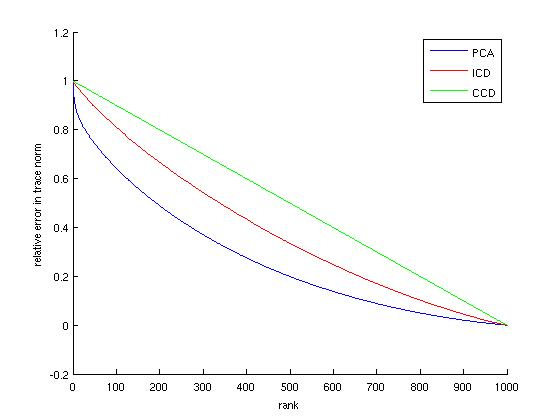
\includegraphics[width=0.5\textwidth]{trace_residual.jpg}
%    \caption{Residual error of decompositions varying by its rank.}
%    \label{fig:residue}
%\end{figure}



\section{Experimental Evaluation}
\subsection{Databases and evaluation protocol} \label{eval:protocol}
Our default database in this report will be INRIA \emph{Holidays} database \cite{holidays}. This database consists of 1491 images divided in 500 groups. For the remaining of this report, if the database of an experiment is not mentioned, the experiment is performed on \emph{Holidays}.
We also perform in the \emph{Oxford} database \cite{oxford}, which consists of 5000 images separated in 55 groups.

Each group of these databases contains one query image. For each query image we rank all the other images in the database based on the similarity between them and the query image, in decreasing order. The average precision of a group is calculated by the ranking of the images of the group for the similarity with the corresponding query image. The final mean average precision (abbreviated for the rest of this report as mAP) for a database is the mean of the average precision over all its groups.
As negative sample of images, we use a small set of images from Flickr100K \cite{oxford}.
\subsection{Base Encoding of Images}
We use three base features as the representation in $\RR^d$ of our images. Firstly, we use VLAD representation, as used in \cite{ZePe15}. 
CNN features are non-negative and can be used both as $\mathbb{L}^1$ or $\mathbb{L}^2$ normalized features. The third features are spatial pyramids of SIFT descriptors, as used in \cite{spk}. These are non-negative $\mathbb{L}^1$ normalized features. \emph{\color{red} Details of these features construction are not relevant right now.}
\subsection{Implementation details}
\emph{\color{red} Not relevant right now.  To be written.}
$8192$ dimensional VLAD features.

E-SVM: $0.6$ second to solve one single exemplar.

SLEM: $30$ seconds to solve a $8192\times 8192$ linear system for all exemplars of the dataset.

Kernelized SLEM: at most $0.3$ seconds (for RBF kernel) for each iteration of (\ref{icd:algo}) algorithm plus at most $30$ seconds to solve a $r'\times r'$ system.

\subsection{Comparison between SLEM and LDA scores}
Let us reconsider the non-kernelized SLEM of subsection \ref{SLEM}. In this case, $A = \frac{1}{n}XX^T-\mu\mu^T+\lambda\textbf{Id}_d$ is the covariance matrix of the negative samples $X$\footnote{A small term proportional to the identity matrix is added to insure the covariance matrix is positive-definite.}. After application of Equation (\ref{beta:fromwood}) to obtain $\omega^\star(x_0,X)$, we can calculate the similarity score $s(x_0,x_0')$ between a query image $x_0$ and an other image $x_0'$ as the inner product of its SLEM vectors:
\begin{equation}
s(x_0,x_0') = (x_0-\mu)^TA^{-2}(x_0'-\mu).
\end{equation}
One interesting fact is that a similar similarity score can be obtained by applying LDA to the positive data. 
Indeed, $\hat{s}(x_0,x_0') = (x_0-\mu)^TA^{-1}(x_0'-\mu)$ is the similarity score for LDA-transformed vectors $x_0$ and $x_0'$. 
\cite{Koba15} noticed that $\hat{s}$ corresponds to the similarity score of SLEM vectors if we use the similarity score proposed in \cite{Efros11} to zero-centered data.

In order to compare both scores, we introduce the similarity score 
\begin{equation}
s_{\alpha}(x_0,x_0') = (x_0-\mu)^TA^{\alpha}(x_0'-\mu),
\end{equation}
and we study how the mAP of \emph{Holidays} evolves when we vary $\alpha$. Notice that $s=s_{-2}$, $\hat{s}=s_{-1}$ and $s_0$ corresponds to zero-centered base features inner product. We also compare both scores to the score obtained by whitening the data (\emph{i.e.}, $\mu$ and $A$ are, respectively, the mean and covariance matrix of the assembled positive and negative data) and by the original base features inner product (\emph{i.e.}, $x_0^Tx_0'$). 
Performing this test on VLAD and CNN feature, as seen on Figure \ref{salpha:vladcnn}, we observe the mAP plateauing for $\alpha$ in $[-2,-1]$, suggesting there is no real improvement in using non-kernelized SLEM over LDA, or, for that matter, the similarity score of \cite{ZePe15}. (which is the most important contribution of this paper) over the similarity of \cite{Efros11}. \emph{\color{red} I'd need to test with E-SVM scores, but if this is true, Patrick's paper is kind of pointless!}
On the other hand, the spatial pyramid features improves its results for smaller values of $\alpha$ in $[-4,0]$, as seen on Figure \ref{salpha:pyr}.
\begin{figure}[!h]
\centering
\begin{subfigure}[b]{0.45\textwidth}
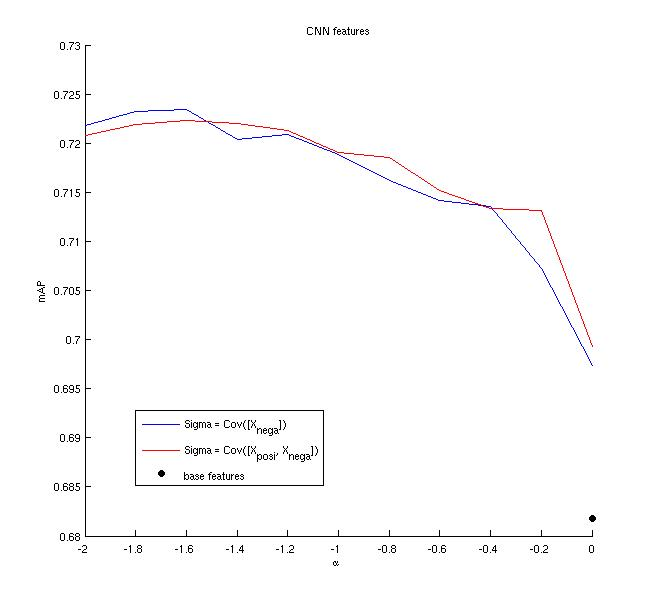
\includegraphics[width=\textwidth]{whitening_cnn.jpg}
\end{subfigure}
\begin{subfigure}[b]{0.45\textwidth}
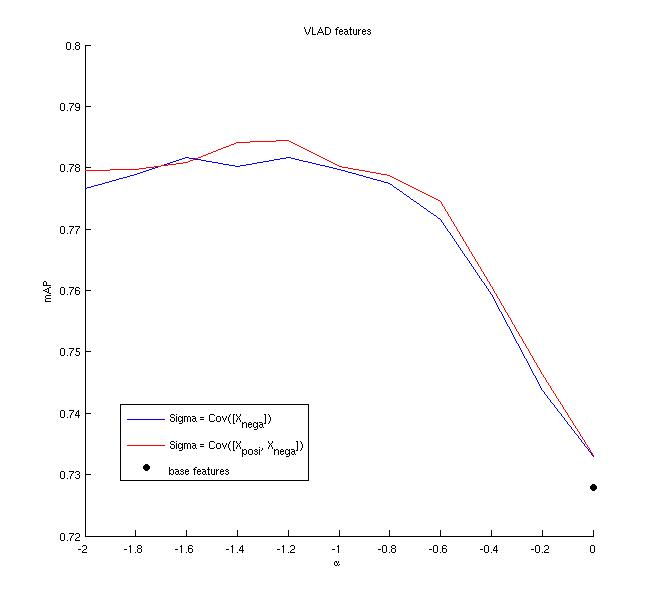
\includegraphics[width=\textwidth]{whitening_vlad.jpg}
\end{subfigure}
\caption{Comparison of mAP for different similarity scores $s_{\alpha}$, varying $\alpha$. On the top, CNN features. At the bottom, VLAD features. On blue, $A$ is the covariance of the negative samples and on red, $A$ is the covariance of the positive and negative samples. In black, the mAP for similarity calculated as inner product of base features.}
\label{salpha:vladcnn}
\end{figure}

\begin{figure}
\centering
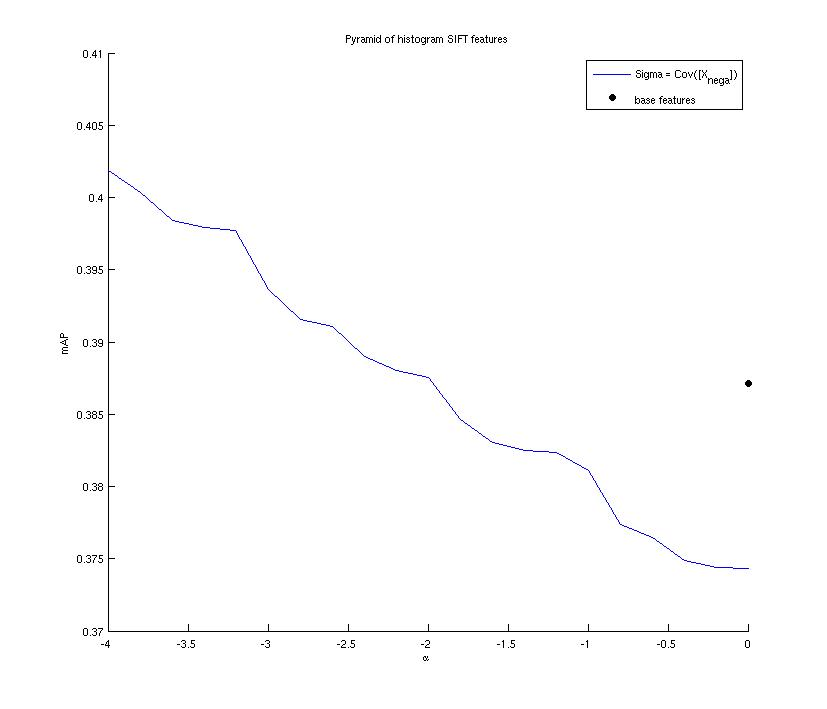
\includegraphics[width=.45\textwidth]{whitening_pyr.jpg}
\caption{Comparison of mAP for different similarity scores $s_{\alpha}$, varying $\alpha$, for spatial pyramid of SIFT descriptors.}
\label{salpha:pyr}
\end{figure}

\begin{table*}[t]
\begin{center}
\begin{tabular}{|l|c|c|c|c|c|}
\hline
Method & $s_0$ & E-SVM \cite{ZePe15} &Linear SLEM & Gaussian SLEM &  Intersection SLEM \\
\hline\hline
VLAD-64 & 73.3 & 77.5 & 77.9 & 78.1 & -\\
Caffe CNN & 69.7 & 71.3 & 72.1 & 72.9 & 70.2\\
Spatial pyramid & 37.4 & 40.1 & 38.2 & 39.7 & 63.5\\
\hline
\end{tabular}
\end{center}
\caption{Results. For all but the second column, we used SLEM. The - means the tests can not be performed or was not performed yet.}
\end{table*}
\subsection{Which kernel to choose?}
For all base features, we test non-kernelized SLEM, as well as kernelized SLEM for Gaussian (rbf):
\begin{align}
k_{rbf}(x,y) &= \exp\left(-\gamma||x-y||^2\right).%;\\
%k_{poly}(x,y) &= x^Ty+\gamma(x^Ty)^2.
\end{align}
For non-negative $\mathbb{L}^1$ normalized, we also test the intersection kernel: 
\begin{equation}
k_{inter}(x,y) = \min(x,y).
\end{equation}
For Gaussian kernel, we can cross validate the parameter $\gamma$. Doing so, we obtained $\gamma$ small ($\gamma\sim 0.5$). Small values of $\gamma$ for the Gaussian kernel mean it is close to the linear kernels, and so its mAP results are not significantly better than the non-kernelized version.

Indeed, if we assume the base features are normalized, i.e. $||x||=||y||=1$, the Taylor series of the exponential function gives us

\begin{align}
k_{rbf}(x,y) &= 1-\gamma||x-y||^2+O(\gamma^2)\\
&=(1-2\gamma)+2\gamma x^Ty+O(\gamma^2)\\
&=C_1+C_2k_{lin}(x,y)+O(\gamma^2).\label{rbf:as:lin}
\end{align}

Equation (\ref{rbf:as:lin}) suggests that for small enough values of $\gamma$, the Gaussian kernel matrix is linearly dependent of the linear kernel matrix. In the context of an image search problem, both kernel matrices give the same result.%\footnote{As explained in section \ref{eval:protocol}, the similarity between positive samples $i$ and $j$ is given by the $j$-th entry of the $i$-th column of the similarity }.


For the spatial pyramid of SIFT, the intersection kernel works much better than all the other kernels. Strangely, this kernel doest not seem to alter the results for CNN features.


\subsection{Low-rank decomposition evaluation}
\emph{\color{red}subsection for the two images on the next page. Important for future work.}
\begin{figure}[!h]
\centering
\includegraphics[width=0.45\textwidth]{None_vs_linear.png}
\caption{Comparison between no kernel results and linear kernel results. In black, mAP of non kernelized SLEM. In red, mAP for different low-rank decompositions of linear kernel matrix. In this experiment, $r=2^{13}$ and we set $\log_2 r'$ in $\{6, 7,...,13\}$. }
\label{no.ker.vs.linear1}
\end{figure}

\begin{figure}[!h]
\centering
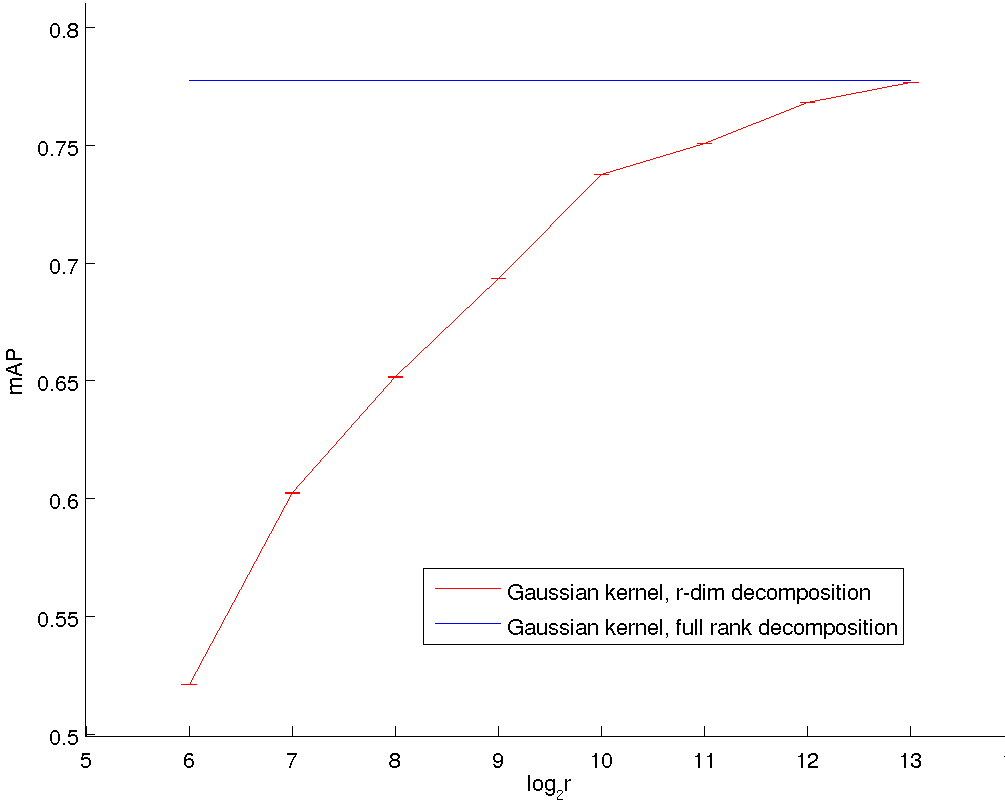
\includegraphics[width=0.45\textwidth]{rbf_decomposition2.png}
\caption{Comparison between no kernel results and linear kernel results. In black, mAP of non kernelized SLEM. In red, mAP for different low-rank decompositions of linear kernel matrix. In this experiment, $r=2^{13}$ and we set $\log_2 r'$ in $\{6, 7,...,13\}$. }
\label{no.ker.vs.linear2}
\end{figure}

\begin{figure}[!h]
\centering
\includegraphics[width=0.45\textwidth]{proj_b_0_2.png}
\caption{}
\label{proj}
\end{figure}
\bibliographystyle{ieee} 
\bibliography{sup}
\end{document}
